\part{Discusión y Conclusiones}

\chapter{Consideraciones del Modelo de PHOEBE} \label{conclusion:consideraciones_phoebe}

El resultado final obtenido en el
\refthesischapter{metodologia:modelocomputacional} está sujeto a varias
consideraciones. En general, es imposible constreñir de manera adecuada varios
parámetros del modelo de un sistema binario estelar utilizando solo curvas
fotométricas resueltas en el tiempo, y aún menos con solo magnitudes
diferenciales. Para tener un modelo más completo se requiere datos
complementarios, como curvas de velocidades radiales para poder obtener el
semi-eje mayor en unidades reales y por ende las masas de ambas
componentes\textemdash cosa que es posible dentro de PHOEBE utilizando
estimadores y optimizadores adicionales a los empleados en este proyecto de
investigación. En este capítulo se plasman detalles particulares con el modelo
sintético derivado, incluyendo degeneraciones en el modelo y un comportamiento
multi-modal que considerar.

\section{Datos Espectroscópicos}

En el transcurso de este proyecto se buscó entre otras fuentes adicionales para
intentar encontrar observaciones espectroscópicas de \atoObjId que pudieran
constreñir otros parámetros del sistema, como la temperatura efectiva del
sistema (la cual se dejaría como parámetro fijo en vez de utilizar la diferencia
de color en el flujo de ZTF) o la masa de la estrella primaria, la cual no se
puede constreñir utilizando solo curvas de luz fotométricas. A pesar de las
capacidades avanzadas de PHOEBE, actualmente no tiene manera de generar un
espectro sintético con cual comparar a un espectro observado. En total se
obtuvieron 3 espectros independientes de \atoObjIdNoSpace : 2 de ellos fueron
proporcionados por la Dra. Paula Szkody de la Universidad de Washington, y 1
espectro obtenido del catálogo Gaia DR3.

\subsection{Apache Point Observatory}

Desde el \textit{Observatorio Apache Point} (\textit{Apache Point Observatory})
la Dra. Szkody logró observar a \atoObjId con el telescopio \textbf{ARC 3.5m}
con el espectrógrafo \textbf{KOSMOS}, un espectrógrafo de baja resolución ($R
\sim 2200$) con una rendija de 0.86 pulgadas en la posición \textit{Alta}, la
cual resulta en un rango de longitudes de onda de $4150 - 7050 \Angstrom$. La
información técnica de KOSMOS se encuentra en la documentación en línea de
KOSMOS\footnote{\url{https://www.apo.nmsu.edu/arc35m/Instruments/KOSMOS/userguide.html}}.
Ambos espectros se pueden ver en la \reffigure{figuraEspectrosApo}.

\begin{figure}[!ht]
    \centering
    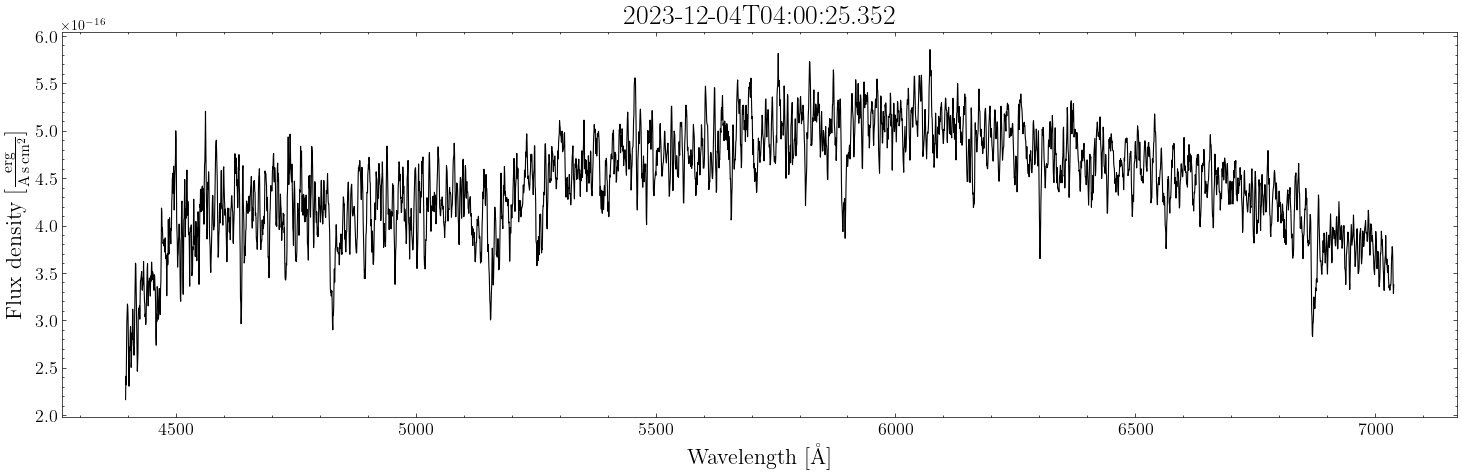
\includegraphics[scale=0.4]{Conclusion/Figures/Figura APO Spectrum 2.png}
    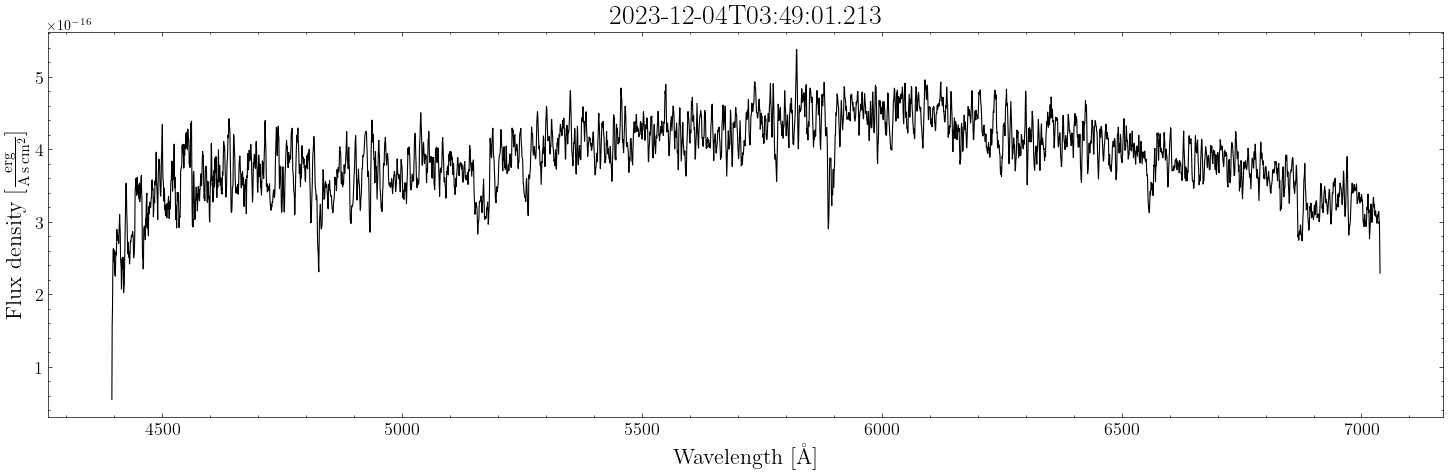
\includegraphics[scale=0.4]{Conclusion/Figures/Figura APO Spectrum 1.png}
    \caption{Espectros tomados de \atoObjId por la Dra. Paula Szkody desde APO.}
    \label{figuraEspectrosApo}
\end{figure}

Los espectros de KOSMOS fueron tomados la misma noche del 4 de diciembre del
2023 en exposiciones de 10 minutos consecutivas. Sin embargo, ambos espectros
muestran una baja razón de señal a ruido (SNR), probablemente por el bajo tiempo
de exposición. Para aumentar el SNR se generó un espectro promedio entre los dos
espectros individuales. Utilizando la función \code{snr\_derived} del paquete
\code{specutils}\footnote{\url{https://specutils.readthedocs.io/en/stable/index.html}}
es posible estimar el SNR basado en solo el espectro medido del archivo. La
función \code{snr\_derived} implementa un algoritmo general para esta tarea,
donde se considera que la señal principal cae en un continuo; el ruido se mide
por la dispersión alrededor del medio del espectro. El espectro promedio se
puede ver en la \reffigure{figuraEspectroApoPromedio}, para el cual el SNR
calculado es de 50.94, a comparación de 39.54 y 38.98 respectivamente de los
espectros individuales en la \reffigure{figuraEspectrosApo}.

\begin{figure}[!ht]
    \centering
    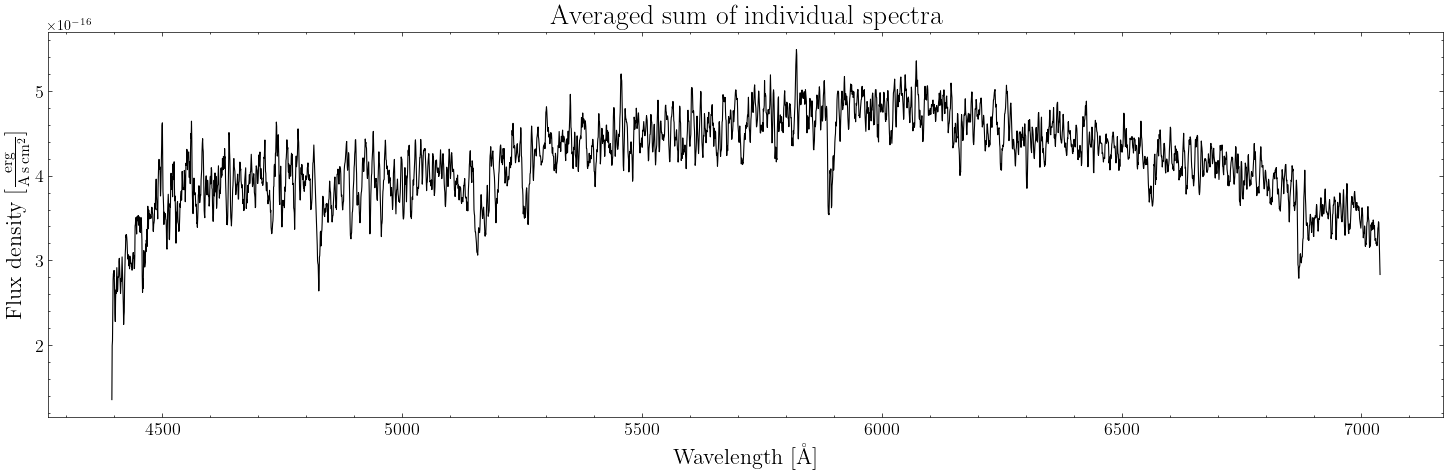
\includegraphics[scale=0.4]{Conclusion/Figures/Figura APO Spectrum Average.png}
    \caption{Espectro promedio de \atoObjIdNoSpace, utilizando el flujo promedio en cada longitud de onda de ambos espectros en la \reffigure{figuraEspectrosApo}.}
    \label{figuraEspectroApoPromedio}
\end{figure}

\subsection{Gaia DR3}

Junto a las curvas de luz fotométricas descritas en la
\refthesissection{muestra:gaia} Gaia DR3 ofrece espectros de aproximadamente 220
millones de las fuentes observadas. Gaia cuenta con un arreglo de
espectro-fotómetros BP y RP (los cuales corresponden a las pasabandas
\textit{Gaia:BP} y \textit{Gaia:RP} respectivamente) que cubren los rangos $[330
- 680] \ \mathrm{nm}$ para BP y $[640 - 1050] \ \mathrm{nm}$ para RP
[\citeyearparen{carrasco_internal_calibration_gdr3_bprp_low_resolution_spectra_2021}].
Cada transito de un objeto por el campo de visión de Gaia contribuye al espectro
promedio de baja resolución; la resolución espectral varía con la longitud de
onda observada, yendo de 100 a 30 para el rango espectral de BP y de 100 a 70
para RP (visto en la figura 3 de
\citeyearparen{carrasco_internal_calibration_gdr3_bprp_low_resolution_spectra_2021}).
Es posible determinar si una fuente en Gaia DR3 cuenta con un espectro por medio
del campo \code{has\_xp\_continuous}. Integrando el espectro en cada rango de
longitud de onda se obtiene el flujo total en Gaia:BP y Gaia:RP.

Para obtener datos limpios de calidad adecuada se someten a un proceso de
calibración extenso, incluyendo la distorsión por la geometría del CCD y la
caracterización del espacio local del objeto\textemdash una revisión extensa del
procesamiento y validación es dada por
\citeyearparen{de_angeli_gdr3_processing_and_validation_bprp_spectra_2023}. El
espectro observado $h_{s,k}(u_i)$ dado un sistema de pseudo-longitudes de onda
$u$ en el catálogo Gaia DR3 se da como una combinación lineal de una función de
base $\varphi$ para una fuente $s$:

\begin{eqfloat}[!ht]
    \begin{equation}
        h_{s,k}(u_i) = \sum_{n=0}^{N - 1} b_{s,n} \sum_{j = -J}^{J} A_k(u_i, u_{i+j}) \varphi_n(u_i+j)
    \end{equation}
\end{eqfloat}

Donde $k$ denota una unidad de calibración (un intervalo de parámetros continuos
cuya variación es baja
[\citeyearparen{carrasco_internal_calibration_gdr3_bprp_low_resolution_spectra_2021}]),
$b_s$ son los coeficientes que contienen la información necesaria para construir
el espectro BP/RP de la fuente, y $A_k$ es el modelo del instrumento. La función
de base elegida por su ortogonalidad, su convergencia a 0 dado un valor de
entrada suficientemente alto, y su centro en $\theta = 0$ se utilizaron
funciones Hermite como las bases del espectro continuo:

\begin{eqfloat}
    \centering
    \begin{equation}
        \begin{split}
            & \varphi_0(\theta) = \pi^{-\frac{1}{4}} e^{-\frac{\theta^2}{2}} \\
            & \varphi_1(\theta) = \sqrt{2} \pi^{-\frac{1}{4}} \theta e^{-\frac{\theta^2}{2}} \\
            & \varphi_n(\theta) = \sqrt{\frac{2}{n}} \theta \varphi_{n-1}(\theta) - \sqrt{\frac{n - 1}{n}} \varphi_{n-2}(\theta)
        \end{split}
    \end{equation}
\end{eqfloat}

Donde se define la transformación lineal de las pseudo-longitudes de onda
$\theta = \Theta \cdot u + \Delta \theta$ con el factor de escala $\Theta$ y un
desplazamiento de $\Delta \theta$ basado en el espectro de la fuente $s$. El
archivo disponible a través del servicio DataLink de Gaia DR3 contiene los
coeficientes de las funciones de base para los espectros BP/RP de
\atoObjIdNoSpace, incluyendo los coeficientes de los errores y la matriz de
correlación entre los coeficientes de las funciones de base. Para facilitar la
lectura y el análisis de este espectro el equipo de Gaia ofrece la herramienta
GaiaXPy\footnote{\url{https://gaiaxpy.readthedocs.io/en/latest/index.html}} que
acepta como entrada el archivo del espectro continuo. Utilizando la función
\code{calibrate} de GaiaXPy este se puede muestrear dado una malla de longitudes
de onda reales en unidades $[\mathrm{nm}]$, dando como resultado el espectro
visto en la \reffigure{figuraEspectroGdr3}.

\begin{figure}[!ht]
    \centering
    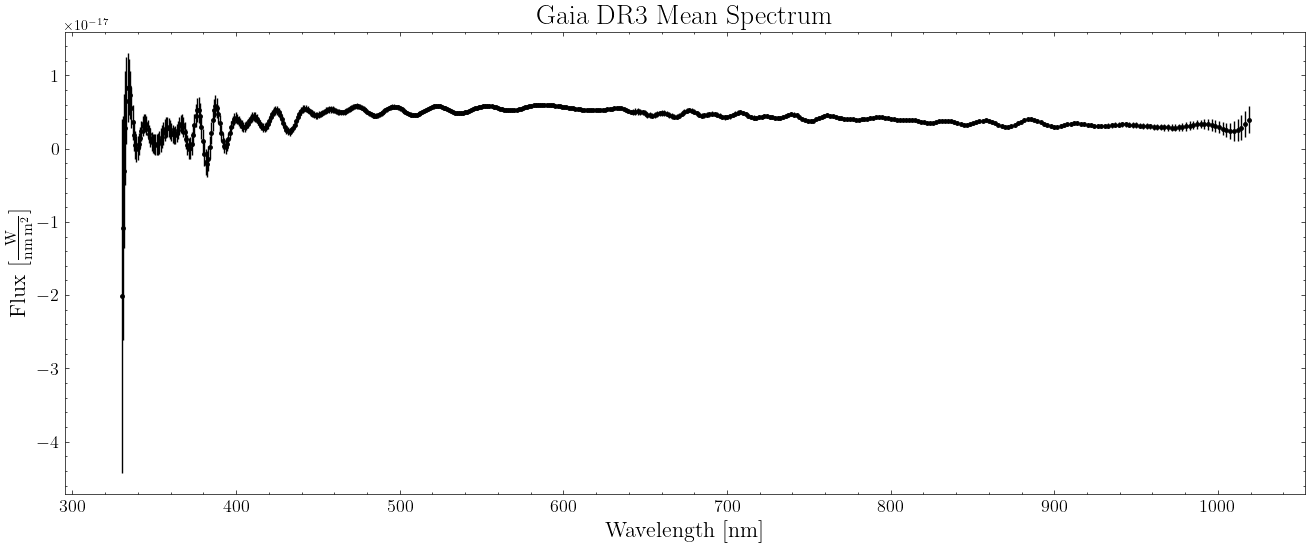
\includegraphics[scale=0.45]{Conclusion/Figures/Figura Gaia DR3 Espectro.png}
    \caption{Espectro continuo de \atoObjId obtenido de Gaia DR3 muestreado
    utilizando una malla de longitudes de onda equidistantes en un espacio
    logarítmico para mejorar la resolución del muestreo en el rango más azul.}
    \label{figuraEspectroGdr3}
\end{figure}

\subsection{Análisis: PyHammer}

Para llevar a cabo un análisis rápido de ambos espectros obtenidos se utilizó la
herramienta de clasificación espectral \textbf{PyHammer}\footnote{Disponible en
GitHub: \url{https://github.com/BU-hammerTeam/PyHammer}}. PyHammer\textemdash
descrito por
\citeyearparen{kesseli_pyhammer1_empirical_template_stellar_spectra_classification_2017}
y después por
\citeyearparen{roulston_pyhammer2_classifying_stars_binaries_stellar_templates_2020}
para la versión 2\textemdash fue desarrollado para facilitar la clasificación
automática y manual de espectros estelares de sistemas binarios por medio de
plantillas espectrales para varios tipos de estrellas, desde tipo O hasta tipo L
generados partiendo de datos del catálogo SDSS BOSS (SDSS Baryon Oscillation
Spectroscopic Survey). Aparte del tipo espectral, PyHammer cuenta con plantillas
para determinar la metalicidad y gravedad superficial (la cual se utiliza para
distinguir entre estrellas enanas y gigantes) basado en líneas espectrales de
referencia. 

Utilizamos ambos espectros especificados en esta sección (el espectro promedio
de APO y el espectro muestreado de Gaia DR3 en una malla de longitudes de onda
uniforme en una escala no logarítmica) para corroborar los parámetros obtenidos
del modelo de PHOEBE. Los resultados de ambos análisis de PyHammer se pueden ver
en la \reffigure{figuraAjustePyHammer}. Ambos resultados indican que el sistema
está compuesto de estrellas tipo K, con una metalicidad de $-0.5 \mathrm{dex}$. 

\begin{figure}[!ht]
    \centering
    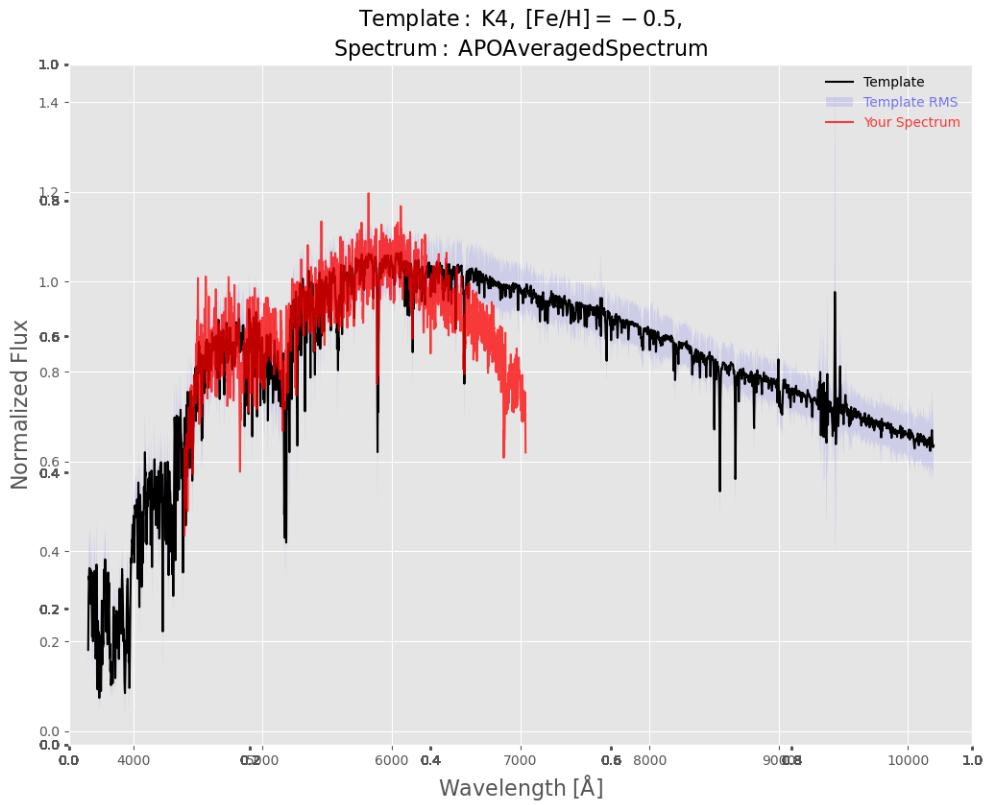
\includegraphics[scale=0.43]{Conclusion/Figures/Figura PyHammer APO.png} \\
    \vspace{0.6em}
    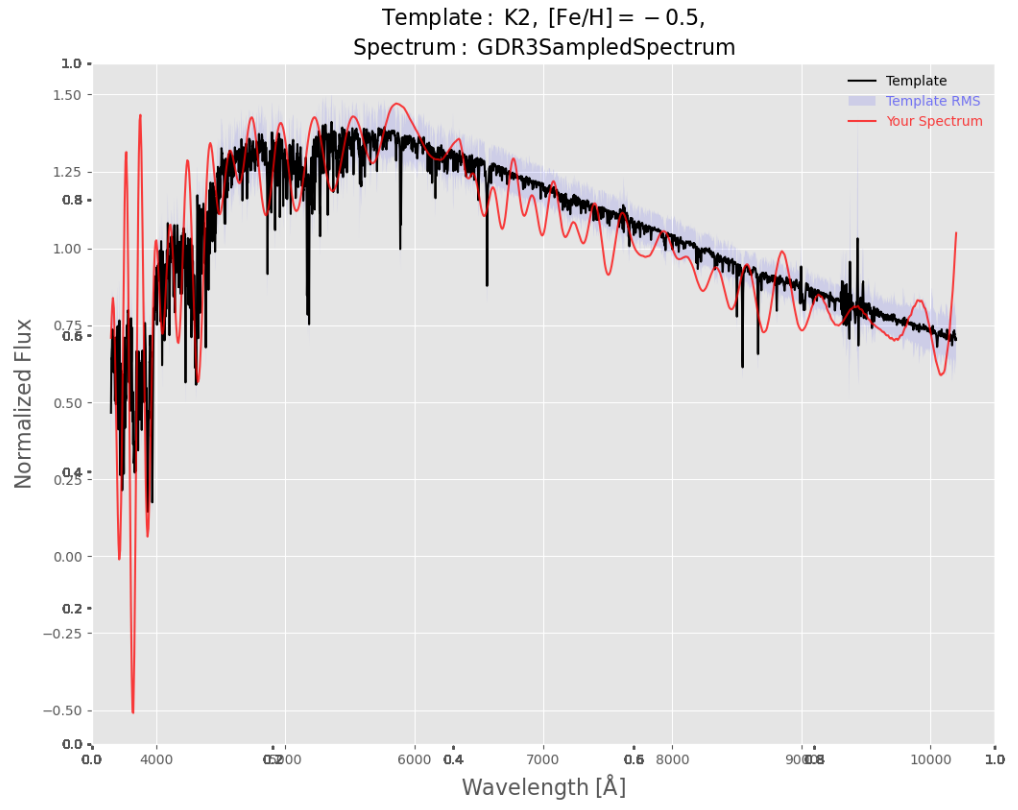
\includegraphics[scale=0.43]{Conclusion/Figures/Figura PyHammer GDR3.png}
    \caption{Resultados del análisis usando PyHammer para el espectro de APO y
    de Gaia DR3 en la gráfica superior e inferior, respectivamente. Partiendo de
    una estimación inicial automática por PyHammer se ajustó el tipo espectral y
    la metalicidad hasta llegar al mejor ajuste visto en esta figura, utilizando
    el $\chi^2$ reportado en la aplicación como guía.}
    \label{figuraAjustePyHammer}
\end{figure}

Los resultados del análisis de PyHammer coinciden con la temperatura efectiva
derivada usando PHOEBE y las curvas fotométricas de ZTF, dado el rango de
temperaturas efectivas de estrellas tipo K de aproximadamente $3900 - 5300 \
\mathrm{K}$. Sin embargo, mucho cuidado es necesario al interpretar estos
resultados. El espectro de Gaia, a pesar de ser el más completo, es de muy baja
resolución espectral, lo cual causa la perdida de información de las líneas de
emisión y absorción que permitirían una clasificación adecuada del sistema. El
espectro de Gaia también muestra errores significativos en las longitudes de
ondas más cortas, lo cual causa una discrepancia contra el espectro de
plantilla. Al mismo tiempo, el espectro de APO carece de una buena razón de
señal a ruido; a pesar de que la plantilla K4 sea la que mejor se ajusta a los
datos, se puede ver en la gráfica superior de la
\reffigure{figuraAjustePyHammer} un decaimiento repentino en las longitudes de
onda más largas del espectro medido, algo que no se observa en el de Gaia y que
no tenemos una explicación satisfactoria en este trabajo. Dado que la
temperatura efectiva de la componente primaria no tiene un efecto significativo
en la morfología de la curva de luz de un sistema binario en contacto
[\citeyearparen{wadhwa_effective_temperature_light_curve_solutions_cbs_2023}] no
es necesario descartar todo el modelo de PHOEBE para \atoObjIdNoSpace. Un
análisis a mayor profundidad con datos espectroscópicos de mayor precisión
ayudaría a constreñir parámetros adicionales del modelo. En el caso de tener
varios espectros del sistema a lo largo del tiempo se podría construir una curva
de velocidades radiales, la cual se podría ingresar al modelo en PHOEBE
directamente.

% TODO: formatting new page
\newpage
\clearpage

\section{Correlaciones Entre Parámetros}

Una de las mayores dificultades en el ajuste de un modelo de un sistema binario
es debido a las correlaciones entre distintos parámetros del modelo. Algunas
correlaciones son esperadas desde un principio; por ejemplo, en un sistema
binario en contacto existe una correlación fundamental entre la razón de masa
$q$ y el factor de escala de la luminosidad en una pasabanda. Un pequeño ejemplo
se puede ver en la \reffigure{figuraRazonMasaLuminosidadSintetico}; esta
relación se manifiesta en una correlación aproximadamente lineal como se puede
ver en la \reffigure{figuraQ_LuminosidadPdfCorrelacion}.

\begin{figure}[!ht]
    \centering
    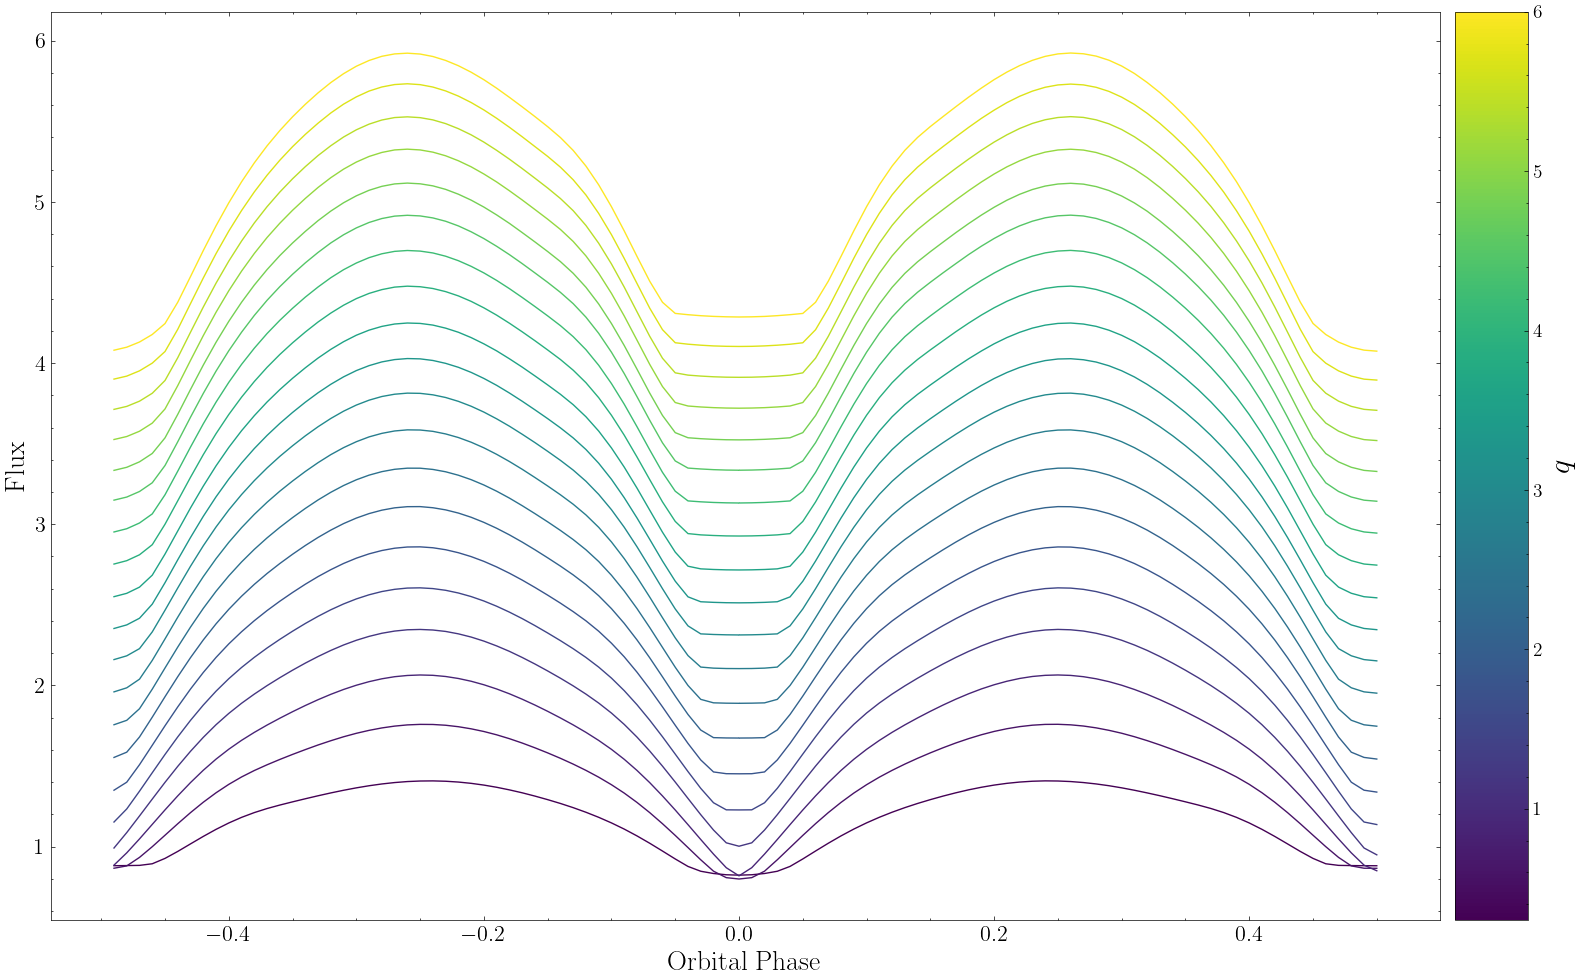
\includegraphics[scale=0.37]{Conclusion/Figures/Figura q-Luminosidad Relacion.png}
    \caption{Modelo sintético en el pasabanda Johnson:V de un sistema binario en
    contacto en PHOEBE, manteniendo fijo el factor de relleno en $f = 0.3$. Se
    puede observar como el flujo sintético calculado va aumentando a pesar de
    mantener fijo el factor de escala de la luminosidad en la
    pasabanda\textemdash la cual corresponde al parámetro
    \code{pblum}\textemdash debido en parte al constreñimiento de los radios
    estelares a la razón de masa.}
    \label{figuraRazonMasaLuminosidadSintetico}
\end{figure}

\begin{figure}[!ht]
    \centering
    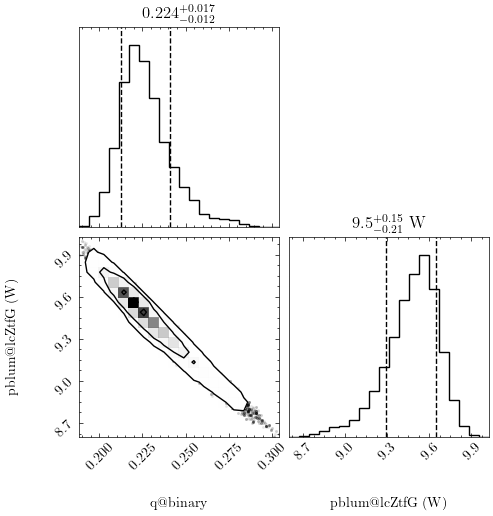
\includegraphics[scale=0.8]{Conclusion/Figures/Figura q-Luminosidad PDF Correlacion.png}
    \caption{Gráfica de correlación entre la razón de masa $q$ y el factor de
    escala de luminosidad en el pasabanda ZTF:g \code{pblum@lcZtfG}.}
    \label{figuraQ_LuminosidadPdfCorrelacion}
\end{figure}

Esta correlación presenta un gran problema para la solución fotométrica del
sistema: los valores presentados en la
\refthesissection{metodologia:modelocomputacional:mcmc:resultados} no
representan una solución única, por la cual cualquier combinación de valores de
la razón de masa y \code{pblum@lcZtfG} que caigan en esta línea pueden llegar a
ajustar el modelo. Esta dependencia se podría eliminar por completo haciendo uso
de flujos absolutos (por ejemplo, el trabajo hecho por
\citeyearparen{odesse_using_computational_models_params_kepler_binaries_2022}),
lo cual por definición dejaría fijo el factor de escala del flujo sintético en
1. Al mismo tiempo esto haría que el modelo sintético sea sensible a cualquier
parámetro que afecte la luminosidad absoluta del sistema, como las masas de las
componentes y temperaturas efectivas, el cual permitiría muestrear estos
parámetros y obtener distribuciones de densidad de probabilidad de ellos.

Para cuantificar las correlaciones entre parámetros se ajustó una relación
polinomio entre los parámetros muestreados. Este proceso se ejecutó para los
pares de parámetros que mostraron una correlación obvia después de una
inspección visual. Se intentó ajustar una función de grado 1 a 10, de los cuales
se hizo un análisis de convergencia para determinar el menor grado del polinomio
que mejor se ajusta a las muestras. La \reffigure{figuraCorrelacion_q_incl}
muestra la correlación entre la razón de masa y la inclinación orbital del
sistema muestreado; las demás correlaciones se pueden ver en el apéndice en la
\refthesissection{apendice:modelo_computacional_graficas:correlaciones_parametros_muestreados}.

\begin{figure}[!ht]
    \centering
    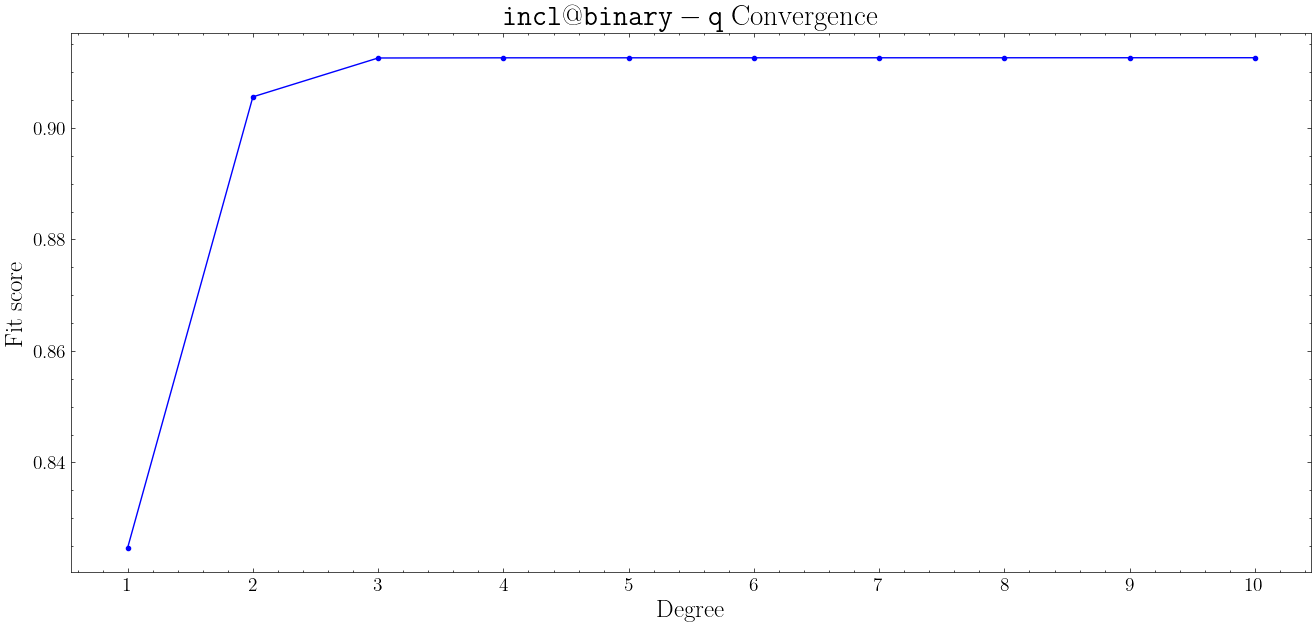
\includegraphics[scale=0.4]{Conclusion/Figures/Figura q-incl Correlacion Convergencia.png}
    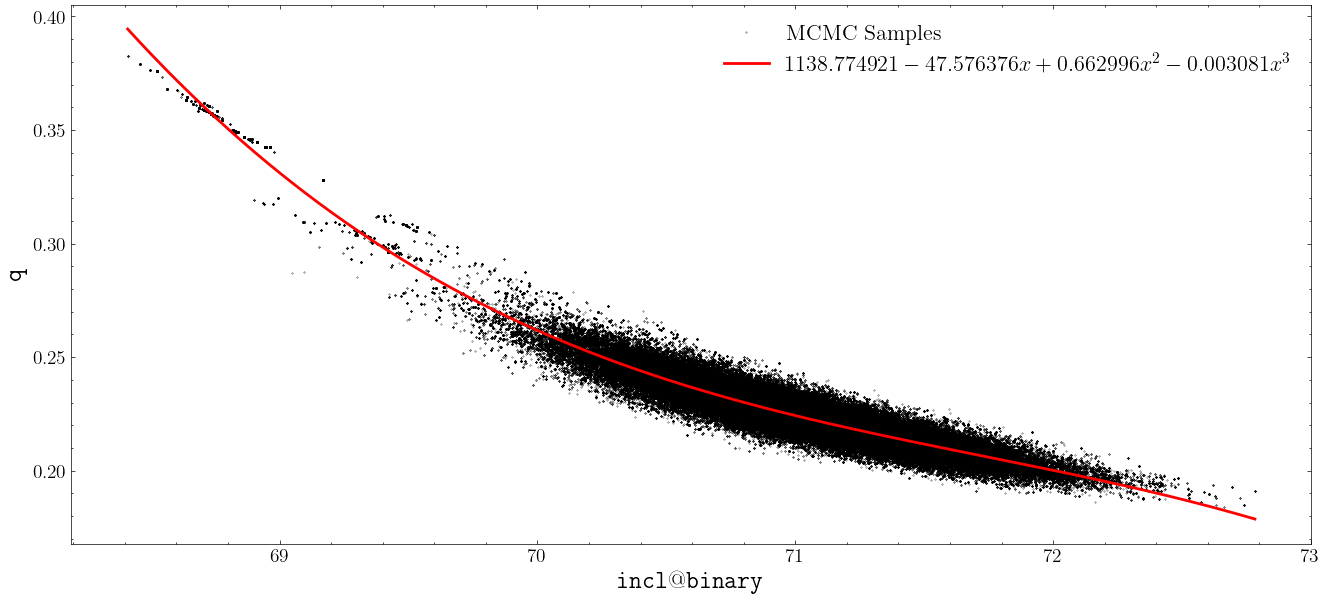
\includegraphics[scale=0.4]{Conclusion/Figures/Figura q-incl Correlacion.png}
    \caption{Función polinomio ajustado a las muestras de la razón de masa
    \code{q} y la inclinación orbital \code{incl@binary}, utilizando los valores
    de la inclinación como el parámetro independiente\textemdash denotado como
    $x$ de la línea solida roja\textemdash para ser consistente con las
    relaciones que aparecen en la \reffigure{figuraMcmcZtfResultadosPrimarios}.
    El ajuste del modelo llega a converger utilizando un polinomio de grado 3 de
    acuerdo a la gráfica superior, el cual es reportado en la gráfica inferior.}
    \label{figuraCorrelacion_q_incl}
\end{figure}

Los ajustes fueron hechos haciendo uso del módulo de regresión lineal de
\href{https://scikit-learn.org/stable/modules/generated/sklearn.linear_model.LinearRegression.html}{\code{scikit-learn}}.
Es importante notar que estas correlaciones aparecen debido a los datos que se
usaron para alimentar el modelo; no es un fenómeno físico presente en el sistema
binario. Cada correlación entre distintos parámetros indica la existencia de una
solución fotométrica no única, dado que cualquier combinación de parámetros que
cumplan con la función de correlación ajustada sería igual de correcta, salvo si
se introducen nuevos datos que permitan restringir aún más los parámetros del
sistema.

% TODO: incluye matriz de covarianza

\section{Extinción Interestelar}

Como se mencionó en la
\refthesissection{metodologia:modelocomputacional:ajuste_luminosidad_teff}, se
utilizó la fotometría de ZTF para determinar la temperatura efectiva del sistema
binario, específicamente los flujos normalizados tal que la información del
color del sistema no se pierda en la conversión de magnitudes. Sin embargo,
cuando se realizó este mismo proceso utilizando los flujos de Gaia DR3 (dados en
cuentas de electrones por segundo), se obtuvo una temperatura efectiva
inconsistente con el resultado de ZTF. Para intentar explicar esta discrepancia
investigamos el efecto de la extinción interestelar debido al polvo en la línea
de visión de \atoObjIdNoSpace.

Para analizar el efecto del polvo en las observaciones fotométricas de Gaia se
utilizó el paquete de Python
\code{dustmaps}\footnote{\url{https://github.com/gregreen/dustmaps}}, el cual
contiene información de varios mapas de polvo hechos en la literatura. Este
paquete contiene mapas que toman en cuenta la distancia al objetivo, calculando
la extinción que experimentaría la luz al pasar por el polvo presente en la
línea de visión. Para este breve análisis se usó el mapa de polvo desarrollado
por \citeyearparen{green_3d_dustmap_gaia_panstarrs_2mass_2019}, el cual utiliza
fotometría de Pan-STARRS 1 y 2MASS en conjunto con las distancias determinadas
utilizando el paralaje reportado en el catálogo de Gaia DR2 para modelar una
distribución tridimensional del polvo interestelar.
\citeyearparen{bailer-jones_estimating_distances_gaia_edr3_2021} corrige errores
sistemáticos en las mediciones del paralaje, reportando distancias corregidas
por medio de métodos probabilísticos, por lo cual decidimos utilizar su
distancia reportada a \atoObjId en vez de una simple inversión del paralaje
reportado por Gaia DR3\footnote{La distancia reportada se encuentra en la tabla
\code{external.gaiaedr3\_distance} en el \textit{Gaia Archive}.}. El mapa de polvo
sintético generado alrededor de \atoObjId se puede ver en la
\reffigure{figuraMapaPolvoLandoltV}.

\begin{figure}[!ht]
    \centering
    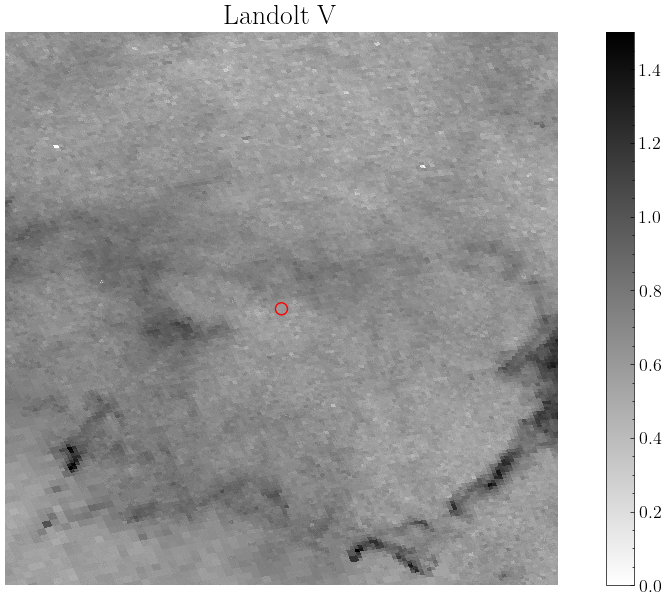
\includegraphics[scale=0.54]{Conclusion/Figures/Figura Mapa Polvo Landolt V.png}
    \caption{Distribución del polvo interestelar alrededor de \atoObjId en la
    pasabanda Landolt V, asumiendo $R_V = 3.1$. Este mapa presenta unidades de
    extinción $A_V$, las cuales se obtuvieron utilizando el coeficiente $2.742$
    reportado por
    \citeyearparen{schlafly_measuring_reddening_sdss_calibrating_sfd_2011}. El
    circulo rojo marca la ubicación de \atoObjIdNoSpace.}
    \label{figuraMapaPolvoLandoltV}
\end{figure}

El exceso $E(B-V)$ es un parámetro libre en PHOEBE, el cual se puede utilizar
para parametrizar el enrojecimiento del sistema binario. Al menos que ambas
componentes estelares sean completamente idénticas y experimenten poca
irradiación mutua y distorsión estelar, no es adecuado tratar la extinción
interestelar como un efecto uniforme en toda la curva de luz de un sistema
binario
[\citeyearparen{jones_phoebe_iv_impact_interstellar_extinction_lcs_binaries_2020}].
PHOEBE es capaz de calcular el valor de la extinción observada en cada fase
orbital basado en el perfil espectral del modelo, la función de transmisión de
el pasabanda de la curva de luz, y la ley de enrojecimiento empleada. Sin
embargo, este método tiene la desventaja de no ser compatible con todas las
pasabandas disponibles en PHOEBE, debido a que uno de los requisitos es que
exista una variación particular \code{ext} en los servidores de PHOEBE. Por esta
razón fue necesario tratar las curvas de luz de Gaia por separado de ZTF.

Primero fue necesario ajustar el tiempo de superconjunción del modelo utilizando
las curvas de luz de Gaia. Esto se debe a la presencia de un efecto sistemático
en el tiempo de medición en la fotometría de Gaia; a pesar de que las curvas se
ajusten adecuadamente al mismo periodo orbital, el eclipse principal del modelo
queda desfasado con los datos observados. Tras correr un optimizador de tipo
Nelder-Mead se encuentra el tiempo de superconjunción de los datos de Gaia de
$0.03199 \ \mathrm{d}$ a comparación de $0.02589 \ \mathrm{d}$ para las curvas
de ZTF e Iturbide. Después fue necesario eliminar la restricción del valor
\code{ebv} del modelo por medio de la función \code{flip\_constraint} del
modelo, restringiendo el valor de \code{Av} en su lugar. Esto nos permite
ingresar de manera directa el valor que se obtiene del exceso en el visible de
\code{dustmaps}, utilizando el módulo \code{BayestarQuery} y usando las
coordenadas de \atoObjId junto a su distancia para obtener una muestra del
enrojecimiento en valores de $E(B-V)$. El valor máximo de $0.16$ logró un mejor
ajuste a los datos, como se puede ver en la
\reffigure{figuraPhoebeGaiaExtinguido}.

\begin{figure}[!ht]
    \centering
    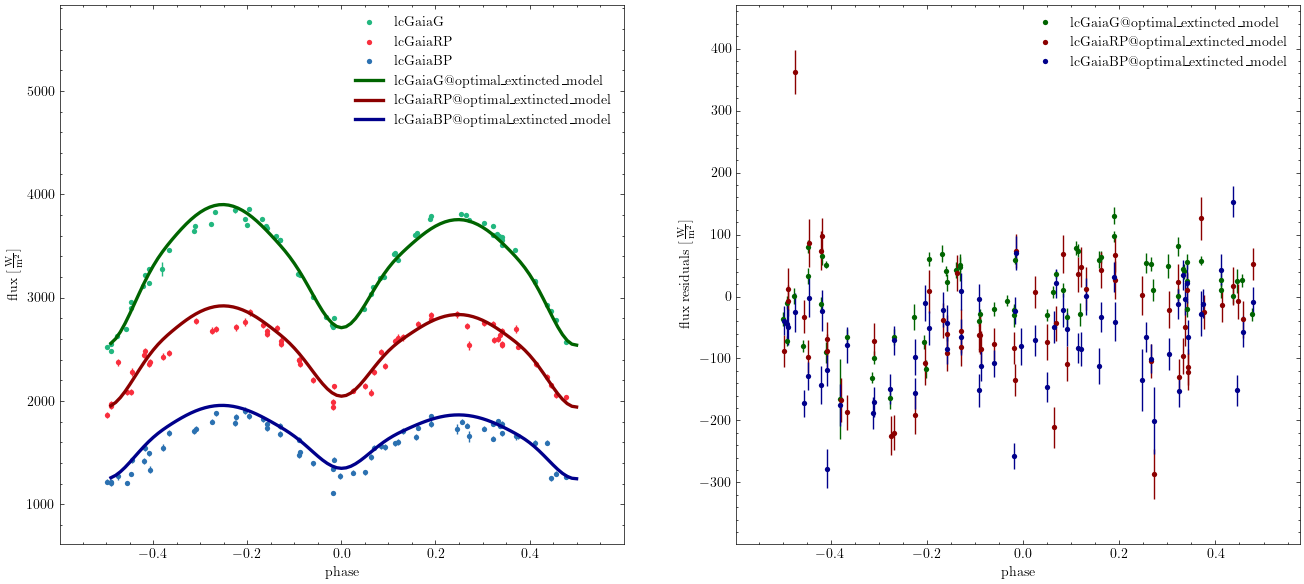
\includegraphics[scale=0.45]{Conclusion/Figures/Figura Phoebe Gaia Extinguido.png}
    \caption{Modelo de PHOEBE incorporando la extinción interestelar a los datos
    de Gaia, utilizando un valor de $0.16$ de $E(B-V)$.}
    \label{figuraPhoebeGaiaExtinguido}
\end{figure}

\section{Multi-Modalidad de la PDF Posterior} \label{conclusion:consideraciones_phoebe:multimodalidad_pdf}

Durante el transcurso de este proyecto se llevaron a cabo varias pruebas e
intentos de ajuste del modelo de PHOEBE a los datos observacionales. El primer
ajuste al que se llegó de manera satisfactoria dio como resultado una
combinación distinta de parámetros; el código relevante se encuentra en una
versión previa en el repositorio de GitHub\footnote{El commit con identificador
18d244a4ac8e5f7e17d0a625156af0e9105245f4 muestra la versión del código más
actual con la solución alterna del modelo.}. Las correlaciones entre parámetros
se pueden ver en la figura \reffigure{figuraAltMcmcResultadosZtf}, junto a los
valores e incertidumbres correspondientes en la
\reftable{tablaMcmcResultadosIncertidumbresAlt}. Para este modelo se adoptaron
diferentes parámetros iniciales de los estimadores corridos\textemdash por
ejemplo, el tiempo de superconjunción se dejó fijo en $-0.0375 \ d$, lo cual
causa que la curva de luz en fase esté centrado en el eclipse más profundo,
afectando el parámetro de razón de temperatura\textemdash lo cual al optimizar y
finalmente muestrear llevó el modelo a una región distinta del espacio de
parámetros. Este muestreo se configuró con 160 caminadores en total, igual que
el muestreo descrito en la
\refthesissection{metodologia:modelocomputacional:mcmc}.

\begin{figure}[!ht]
    \centering
    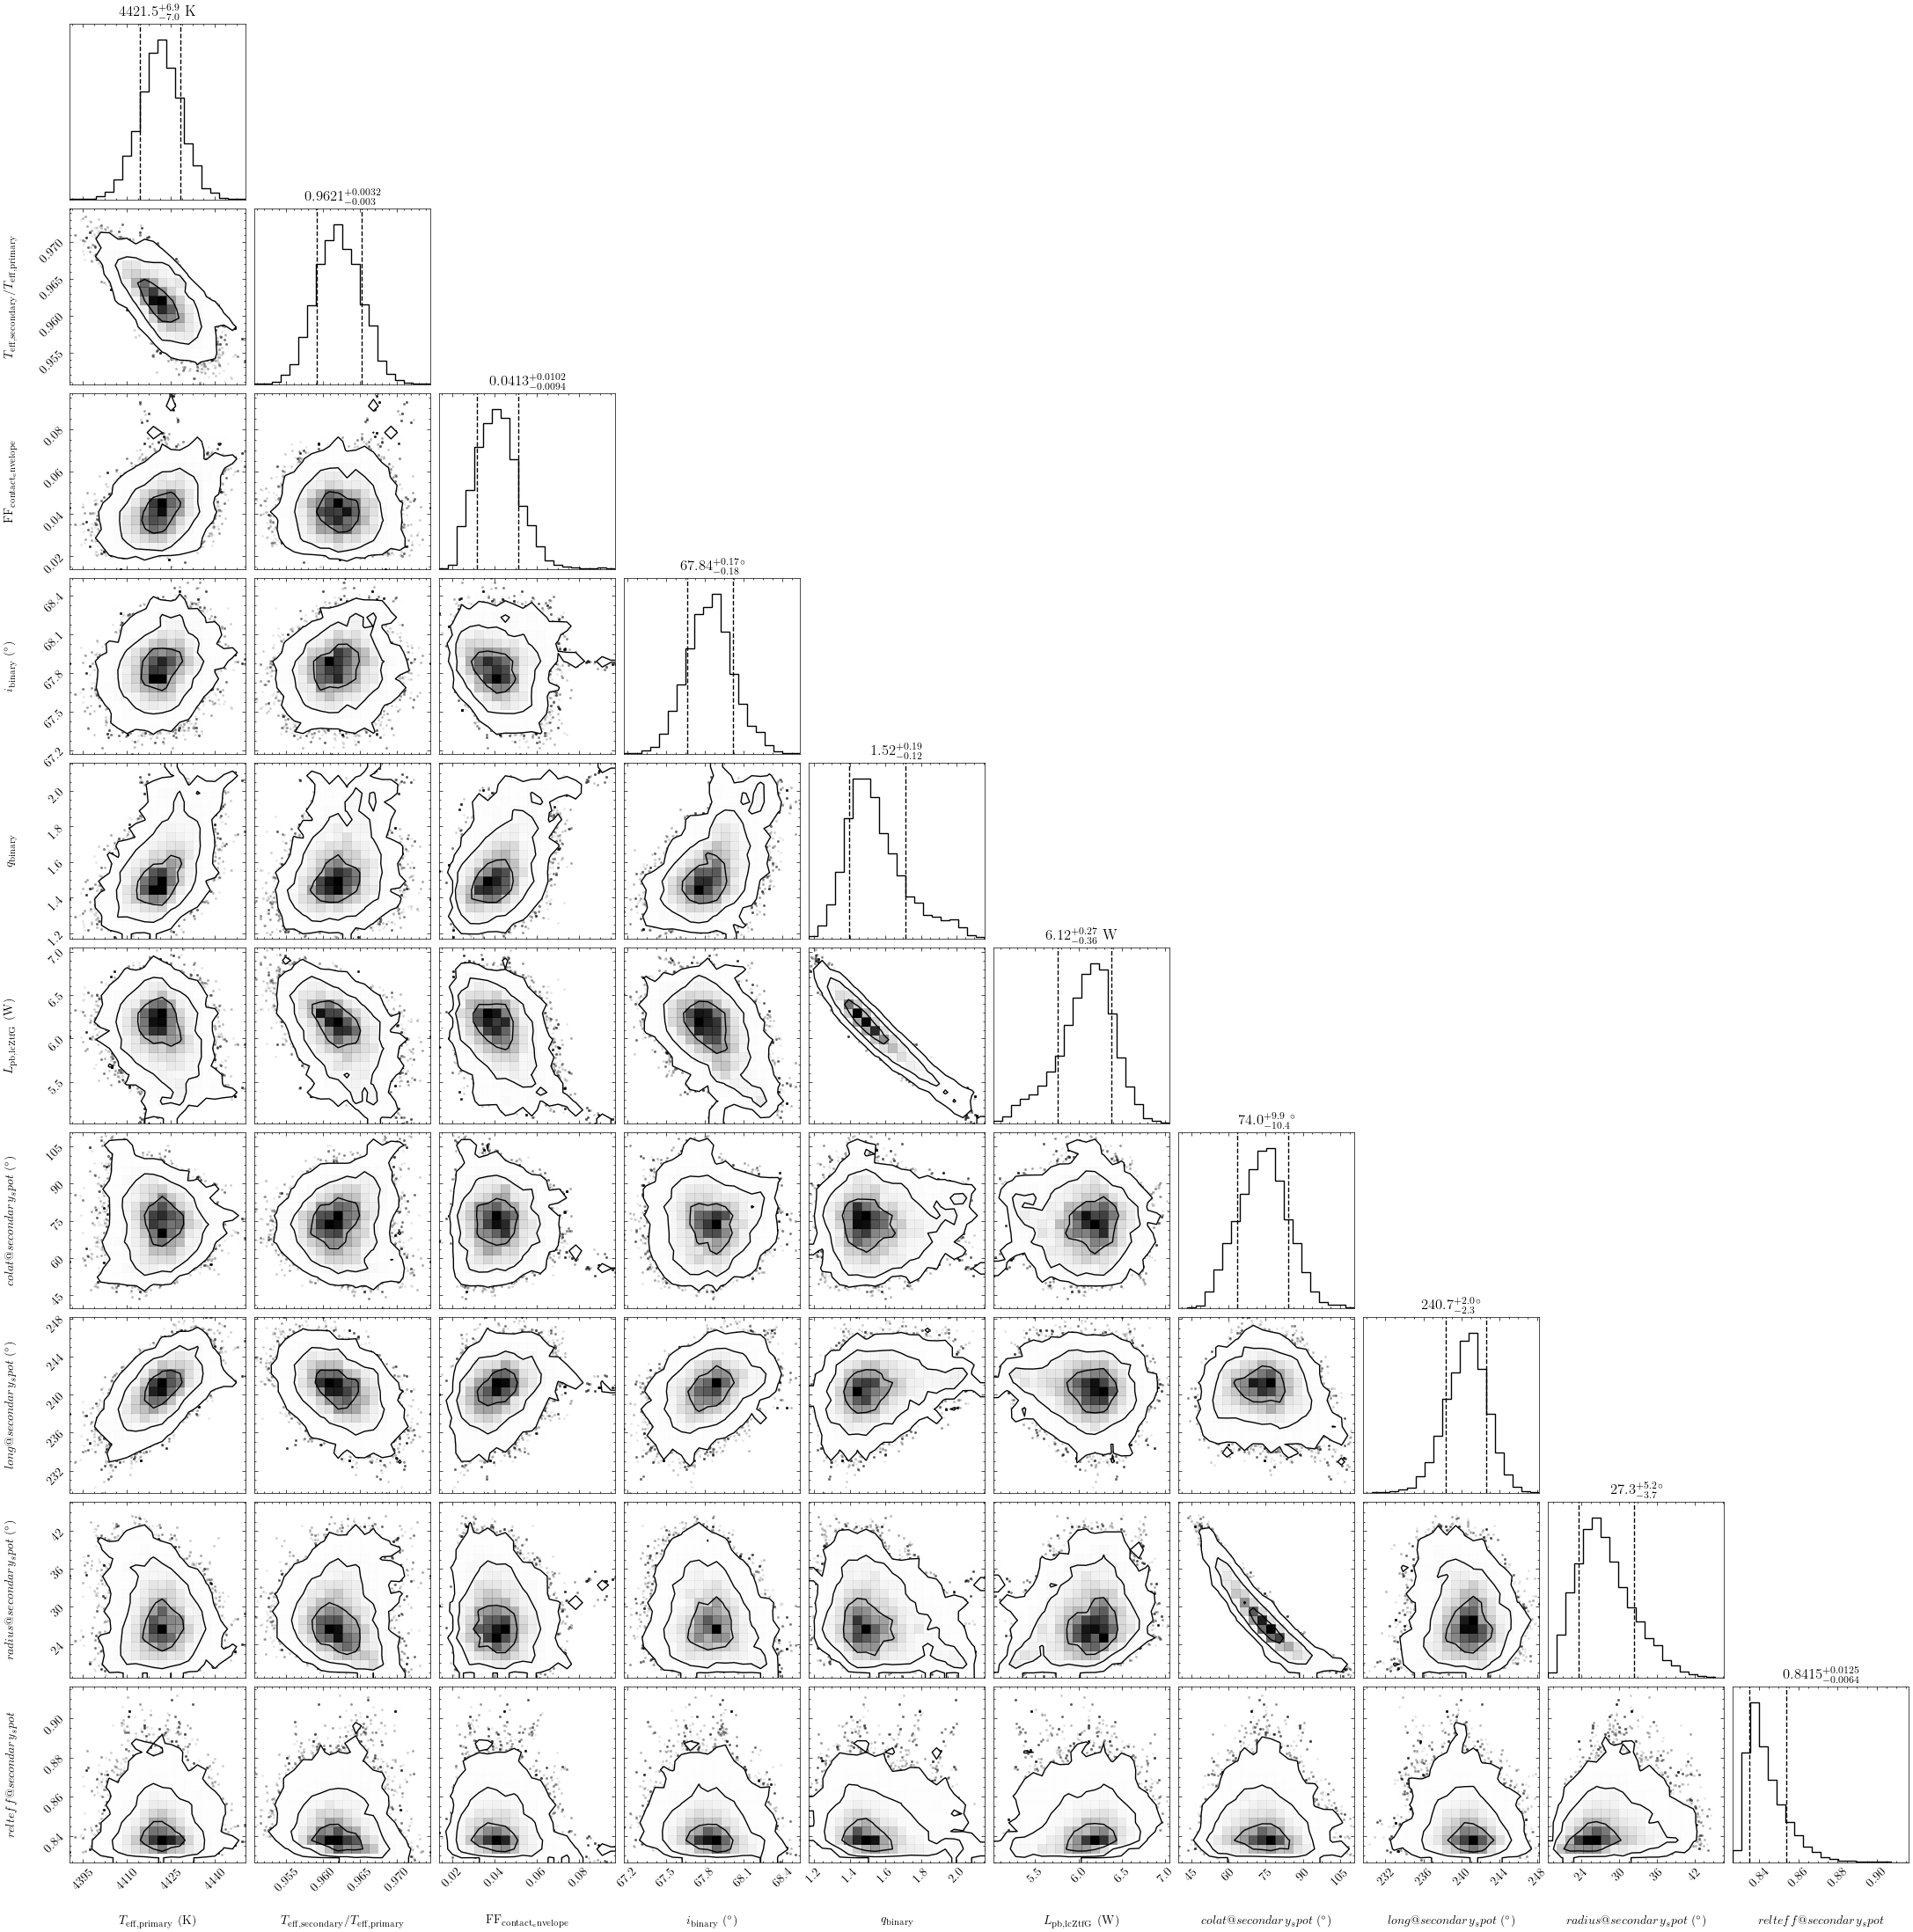
\includegraphics[scale=0.27]{Conclusion/Figures/Figura Alt Solucion MCMC ZTF.png}
    \caption{Gráfica de correlación de una solución alterna que se obtuvo
    utilizando las curvas de ZTF. Incluye el parámetro de molestia
    \code{pblum@lcZtfG}.}
    \label{figuraAltMcmcResultadosZtf}
\end{figure}

{\renewcommand{\arraystretch}{1.5}%
\begin{table}[!ht]
	\centering
	\begin{tabular}{|P{3cm}|P{4cm}|}
		\hline
		\thead{Parámetro}                        & \thead{Valor} \\
		\hline
        $T_{1}$ & $4421.5^{ +6.9 }_{ -7.0 } ~\mathrm{K}$ \\
        \hline
        $T_2 / T_1$ & $0.9621^{ +0.0032 }_{ -0.003 } \mathrm{}$ \\
        \hline
        $f$ & $0.0413^{ +0.0102 }_{ -0.0094 } \mathrm{}$ \\
        \hline
        $i_{\mathrm{orb}}$ & $67.84^{ +0.17 }_{ -0.18 } \mathrm{{}^{\circ}}$ \\
        \hline
        $q$ & $1.52^{ +0.19 }_{ -0.12 } \mathrm{}$ \\
        \hline
        $\mathrm{ Lat }_{\mathrm{spot}}$ & $74.0^{ +9.9 }_{ -10.4 } \mathrm{{}^{\circ}}$ \\
        \hline
        $\mathrm{ Lon }_{\mathrm{spot}}$ & $240.7^{ +2.0 }_{ -2.3 } \mathrm{{}^{\circ}}$ \\
        \hline
        $\mathrm{ Radius }_{\mathrm{spot}}$ & $27.3^{ +5.2 }_{ -3.7 } \mathrm{{}^{\circ}}$ \\
        \hline
        $T_{\mathrm{spot}} / T_2$ & $0.8415^{ +0.0125 }_{ -0.0064 } \mathrm{}$ \\
        \hline
	\end{tabular}
	\caption{Valores e incertidumbres de solución alterna al modelo de PHOEBE.}
	\label{tablaMcmcResultadosIncertidumbresAlt}
\end{table}}

Esta solución fue obtenida después de 6116 iteraciones en total. Sin embargo,
esta solución no es completamente adecuada. El periodo de quemado fue de 4816;
esto se debe a que los caminadores se encontraban atrapados en ciertas regiones
del espacio de parámetros, nunca saliendo por su propia cuenta. La solución para
este problema fue utilizar la capacidad del resolvedor MCMC de PHOEBE para
adoptar el resultado del muestreo como las distribuciones priori de un nuevo
muestreo MCMC. Con el fin de eliminar las muestras de los caminadores inmóviles
se aproximaron las distribuciones posteriores de muestras a distribuciones
continuas Gaussianas multi-dimensionales; a pesar de perder información de la
forma discreta de las muestras\textemdash y al mismo tiempo introduce un sesgo
en la forma inicial de las muestras\textemdash dados suficiente iteraciones los
caminadores tendrán la oportunidad de explorar el espacio fuera de la región
dada por las distribuciones a priori, siguiendo la forma de la distribución
posterior. Debido a que solo se pudieron correr un total de 1345 para la última
ronda de muestreo (el cual incluye 304 iteraciones del periodo de quemado, lo
que eleva el tiempo de quemado total a 5120 iteraciones con solo 996 iteraciones
utilizadas) no es posible decir que este muestreo ha convergido de manera
adecuada.

Debido a la falta de experiencia utilizando PHOEBE, la optimización del tiempo
de cómputo de este muestreo inicial se llevó a cabo de una manera distinta. A
parte del proceso de eliminación de observaciones erróneas que se realizó
(descrito en la
\refthesissubsection{metodologia:modelocomputacional:mcmc:eliminacion_errores}),
se eliminaron la mitad de las observaciones de ambas curvas ZTF:g y ZTF:r,
utilizando los \quotes{slices} de Python. A pesar de que este método redujo el
tiempo de cómputo del modelo hacia adelante, tiene la desventaja de perder mucha
información de observaciones individuales. Al mismo tiempo, esta optimización no
tuvo el mismo efecto significativo que solo computar el modelo hacia adelante
para una malla de fases orbitales determinadas (descrito en la
\refthesissection{metodologia:modelocomputacional:preparacion_modelo}), lo cual
resultó en tiempos promedios de $\sim 3600 \ \mathrm{seg}$ por iteración de MCMC
contra un tiempo promedio de $\sim 500 \ \mathrm{seg}$ por iteración del último
muestreo descrito en la \refthesissection{metodologia:modelocomputacional:mcmc}. 

Este primer intento de explorar el espacio de parámetros se ejecutó en el
servidor \quotes{Alziir} por parte del Instituto de Astronomía Ensenada de la
Universidad Nacional Autónoma de México, en colaboración con el Dr. Raúl Michel
Murillo. Esta computadora cuenta con un procesador AMD Opteron(tm) Processor
6376 de 64 hilos, con un total de 512 GB de memoria RAM; una vez corriendo el
código en el servidor, el proceso llegó a ocupar más de 50 GB de memoria. Debido
al alto tiempo de cómputo para cada iteración, y la solución alterna dada en la
\refthesissubsection{metodologia:modelocomputacional:mcmc:resultados}, esta
solución se abandonó por el momento, pero debería de ser considerada en un
trabajo a futuro en caso que se obtenga una nueva fuente de datos para
constreñir el modelo. 

\chapter{Conclusiones}

Se ha presentado la búsqueda de sistemas binarios eclipsantes dentro del
catálogo de Gaia DR3 con el objetivo de realizar una campaña de observación
fotométrica desde el Observatorio Astronómico Universitario en Iturbide, N.L.
\atoObjId fue elegido como el objetivo de interés debido a su clasificación como
\textit{candidata a binaria eclipsante} durante el tiempo en el que se realizó
la búsqueda de objetos. Este objeto de magnitud 16.91 en la banda $G$ de Gaia
fue observado en el rango óptico por 9 noches utilizando el telescopio CDK20 de
0.5m de diámetro. Esta campaña de observación resultó en una curva de luz
fotométrica de \atoObjIdNoSpace, también sirviendo como una prueba de la
factibilidad de campañas de observación de sistemas binarios tenues desde el
OAU-Iturbide.

Para complementar los datos disponibles de \atoObjId se obtuvieron curvas
fotométricas adicionales obtenidas de los catálogos de ZTF DR20 y Gaia DR3 con
el objetivo de realizar un estudio fotométrico particular del objeto de interés.
Primero se encontró el periodo orbital del sistema de $8.00558 \pm 0.00013 \
\mathrm{h}$. Partiendo del corto periodo orbital del sistema junto a la
morfología aparente de las curvas de luz en fase se ajustó un modelo de un
sistema binario eclipsante en contacto utilizando PHOEBE, del cual al final se
obtuvieron una parte de los parámetros fundamentales estelares y orbitales del
sistema, descritos en la
\refthesissection{metodologia:modelocomputacional:resultados}. Algunas
consideraciones de estos resultados\textemdash incluyendo un análisis
rudimentario de datos espectroscópicos adicionales y una posible solución
fotométrica alterna dada en la
\refthesissection{conclusion:consideraciones_phoebe:multimodalidad_pdf}\textemdash
se presentó para resaltar las limitaciones de la solución fotométrica presentada
en este trabajo\textemdash cosa que puede ser posible eliminar con la inclusión
de datos espectroscópicos adicionales (ie. curvas de velocidades radiales o
distribuciones de energía espectral de las componentes)\textemdash y las
correlaciones presentes entre los distintos parámetros del modelo.